\documentclass{beamer}
\usepackage{tikz,amsmath,hyperref,graphicx,stackrel,animate,media9}
\usetikzlibrary{positioning,shadows,arrows,shapes,calc}
\newcommand{\argmax}{\operatornamewithlimits{argmax}}
\newcommand{\argmin}{\operatornamewithlimits{argmin}}
\mode<presentation>{\usetheme{Frankfurt}}
\AtBeginSection[]
{
  \begin{frame}<beamer>
    \frametitle{Outline}
    \tableofcontents[currentsection,currentsubsection]
  \end{frame}
}
\title{Lecture 8: Filtering Periodic Signals}
\author{Mark Hasegawa-Johnson}
\date{ECE 401: Signal and Image Analysis, Fall 2020}  
\begin{document}

% Title
\begin{frame}
  \maketitle
\end{frame}

% Title
\begin{frame}
  \tableofcontents
\end{frame}

%%%%%%%%%%%%%%%%%%%%%%%%%%%%%%%%%%%%%%%%%%%%
\section[Review]{Review: Frequency Response}
\setcounter{subsection}{1}

\begin{frame}
  \frametitle{What is Signal Processing, Really?}

  \begin{itemize}
  \item When we process a signal, usually, we're trying to
    enhance the meaningful part, and reduce the noise.
  \item {\bf Spectrum} helps us  to understand which part is
    meaningful, and which part is noise.
  \item {\bf Convolution} (a.k.a. filtering) is the tool we use to
    perform the enhancement.
  \item {\bf Frequency Response} of a filter tells us exactly which
    frequencies it will enhance, and which it will reduce.
  \end{itemize}
\end{frame}

\begin{frame}
  \frametitle{Review: Convolution}
  \begin{itemize}
  \item A {\bf convolution} is exactly the same thing as a {\bf weighted local average}.
    We give it a special name, because we will use it very often.  It's defined as:
    \[
    y[n] = \sum_m g[m] f[n-m] = \sum_m g[n-m] f[m]
    \]
  \item 
    We use the symbol $\ast$ to mean ``convolution:''
    \[
    y[n]=g[n]\ast f[n] = \sum_m g[m] f[n-m] = \sum_m g[n-m] f[m]
    \]
  \end{itemize}
\end{frame}

\begin{frame}
  \frametitle{Review: DFT \& Fourier Series}

  The most useful type of spectrum is a Fourier series (in discrete
  time: a DFT).  {\bf\em Any} periodic signal with a period of $N$
  samples, $x[n+N] = x[n]$, can be written as
  \[
  x[n] = \frac{1}{N}\sum_{k=0}^{N-1} X[k] e^{j2\pi kn/N}
  \]
  which is a special case of the spectrum for periodic signals:
  \[
  \omega_0=\frac{2\pi}{N}\frac{\mbox{radians}}{\mbox{sample}},~~~
  F_0=\frac{1}{T_0}\frac{\mbox{cycles}}{\mbox{second}},~~~
  T_0=\frac{N}{F_s}\frac{\mbox{seconds}}{\mbox{cycle}},~~~
  N = \frac{\mbox{samples}}{\mbox{cycle}}
  \]
  and
  \[
  X[k] = \sum_{n=0}^{N-1} x[n]e^{-j2\pi kn/N}  
  \]
\end{frame}


\begin{frame}
  \frametitle{Frequency Response}
  \begin{itemize}
  \item {\bf Tones in $\rightarrow$ Tones out}
    \begin{align*}
      x[n]=e^{j\omega n} &\rightarrow y[n]=G(\omega)e^{j\omega n}\\
      x[n]=\cos\left(\omega n\right)
      &\rightarrow y[n]=|G(\omega)|\cos\left(\omega n+\angle G(\omega)\right)\\
      x[n]=A\cos\left(\omega n+\theta\right)
      &\rightarrow y[n]=A|G(\omega)|\cos\left(\omega n+\theta+\angle G(\omega)\right)
    \end{align*}
  \item where the {\bf Frequency Response} is given by
    \[
    G(\omega) = \sum_m g[m]e^{-j\omega m}
    \]
  \end{itemize}
\end{frame}  

%%%%%%%%%%%%%%%%%%%%%%%%%%%%%%%%%%%%%%%%%%%%
\section[Delta]{Delta Function: the  ``Do-Nothing Filter''}
\setcounter{subsection}{1}

\begin{frame}
  \frametitle{Delta: the do-nothing filter}

  First, let's define a do-nothing filter, called $\delta[n]$:
  \[
  \delta[n] = \begin{cases}
    1 & n=0\\
    0 & n\ne 0
  \end{cases}
  \]
  Its frequency response is
  \[
  \sum_m \delta[m]e^{-j\omega m} = 1
  \]
  This has the property that, when you convolve it within anything, you get that thing back again:
  \[
  x[n]\ast \delta[n] = x[n]
  \]
\end{frame}

%%%%%%%%%%%%%%%%%%%%%%%%%%%%%%%%%%%%%%%%%%%%
\section[Pure Delay]{A Pure-Delay ``Filter''}
\setcounter{subsection}{1}

\begin{frame}
  \frametitle{A Pure-Delay ``Filter''}

  One thing we can do to a signal is to just delay it, by $n_0$ samples:
  \[
  y[n] = x[n-n_0]
  \]
  Even this very simple operation can be written as a convolution:
  \[
  y[n]=g[n]\ast x[n]
  \]
  where the ``filter,'' $g[n]$, is just
  \[
  g[n]=\delta[n-n_0] = \begin{cases}
  1 & n=n_0\\
  0 & \mbox{otherwise}
  \end{cases}
  \]
\end{frame}

\begin{frame}
  \frametitle{Impulse Response of A Pure-Delay ``Filter''}
  Here is the impulse response of a pure-delay ``filter'' (and the magnitude and
  phase responses, which we'll talk about next).
\centerline{\includegraphics[height=2.5in]{exp/puredelay.png}}
\end{frame}

\begin{frame}
  \frametitle{Frequency Response of A Pure-Delay ``Filter''}

  \[
  g[n]=\begin{cases}
  1 & n=n_0\\
  0 & \mbox{otherwise}
  \end{cases}
  \]
  The frequency response is
  \[
  G(\omega)=\sum_m g[m]e^{-j\omega m} = e^{-j\omega n_0}
  \]
  
\end{frame}

\begin{frame}
  \frametitle{Magnitude and Phase Response of A Pure-Delay ``Filter''}

  \[
  G(\omega)=\sum_m g[m]e^{-j\omega m} = e^{-j\omega n_0}
  \]
  Notice that the magnitude and phase response of this filter are
  \begin{align*}
    |G(\omega)| &= 1\\
    \angle G(\omega) &= -\omega n_0
  \end{align*}
  So, for example, if have an input of $x[n]=\cos(\omega n)$, the
  output would be
  \[
  y[n]=|G(\omega)|\cos\left(\omega n+\angle G(\omega)\right)
  = \cos\left(\omega n-\omega n_0\right)
  \]
\end{frame}

\begin{frame}
  \frametitle{Magnitude and Phase Response of A Pure-Delay ``Filter''}
  Here are the magnitude and phase response of the pure delay filter.
\centerline{\includegraphics[height=2.5in]{exp/puredelay.png}}
\end{frame}

\begin{frame}
  \frametitle{Spectrum of a Square Wave}

  Let's prove that the ``pure delay'' filter changes the phase
  spectrum, but has no influence on the magnitude spectrum.  As the input,
  here's an (almost) square wave,
  with a period of 11 samples:
  \centerline{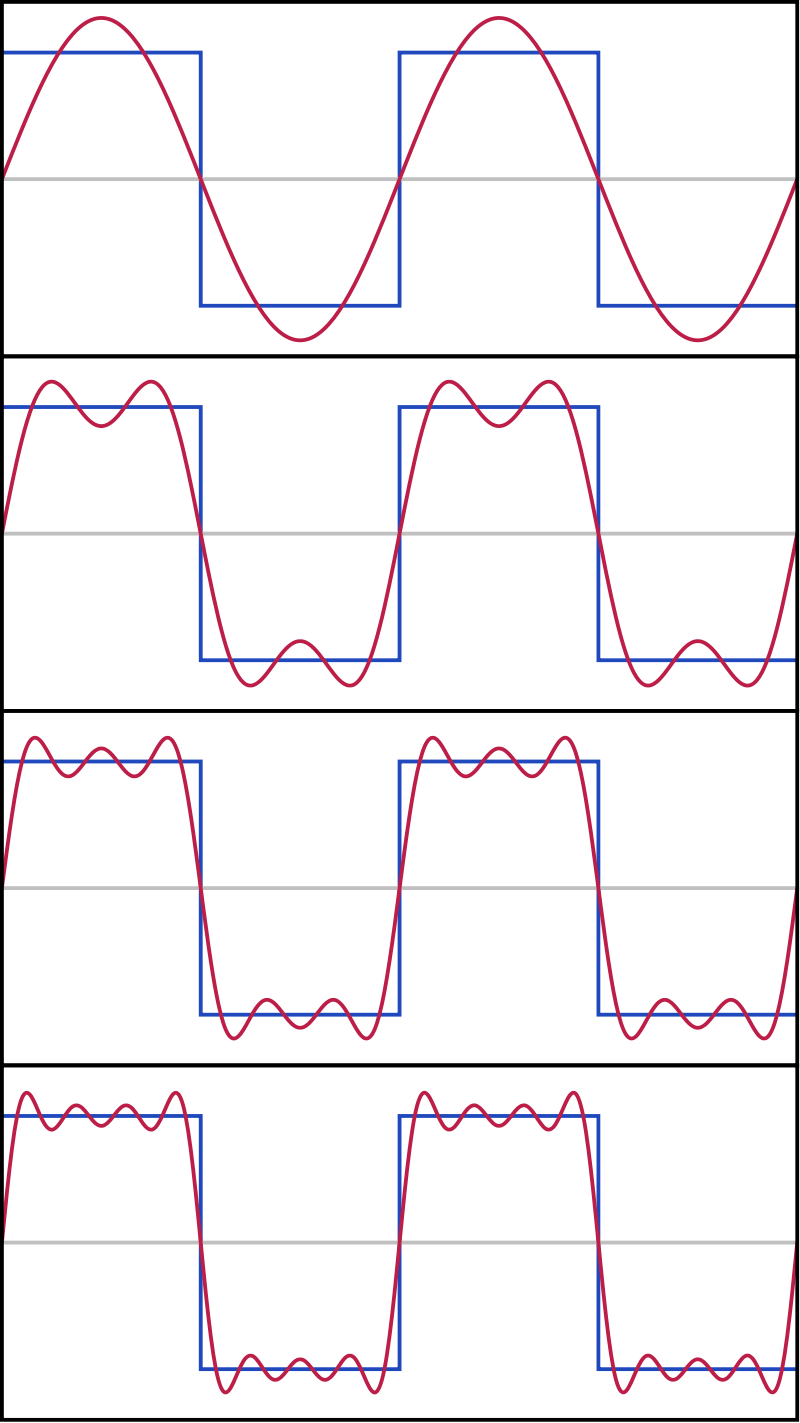
\includegraphics[height=2.5in]{exp/squarewave.png}}
\end{frame}

\begin{frame}
  \frametitle{More about the phase spectrum}
  \centerline{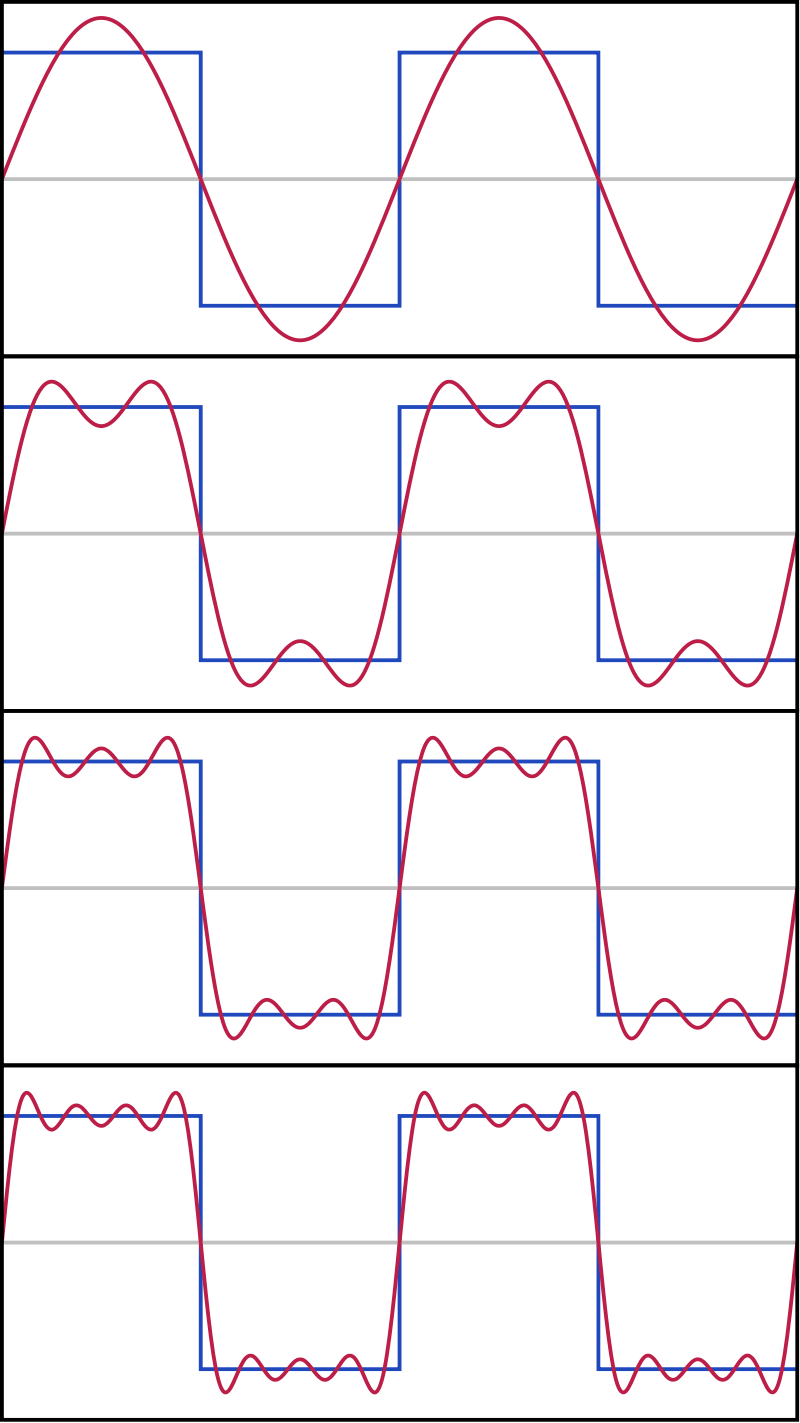
\includegraphics[height=1.5in]{exp/squarewave.png}}
  Notice that, for the phase spectrum of a square wave, the phase
  spectrum is either $\angle X[k]=0$ or $\angle X[k]=\pi$.  That means that the
  spectrum is real-valued, with no complex part:
  \begin{itemize}
  \item {\bf Positive real:} $X[k]=|X[k]|$
  \item {\bf Negative real:} $X[k]=-|X[k]| = |X[k]|e^{j\pi}$
  \end{itemize}
\end{frame}

\begin{frame}
  \frametitle{More about the phase spectrum}
  
  Having discovered that the square wave has a real-valued $X[k]$, we could
  just plot $X[k]$ itself, instead of plotting its magnitude and phase:
  \centerline{\includegraphics[height=2.5in]{exp/squarewave_real.png}}
\end{frame}

\begin{frame}
  \frametitle{More about the phase spectrum}

  But delaying the signal to compute $y[n]=x[n-5]$ is going to change
  the phase, so $Y[k]$ won't be real-valued.  In preparation for
  $Y[k]$, let's go back to plotting the magnitude and phase
  separately:
  \centerline{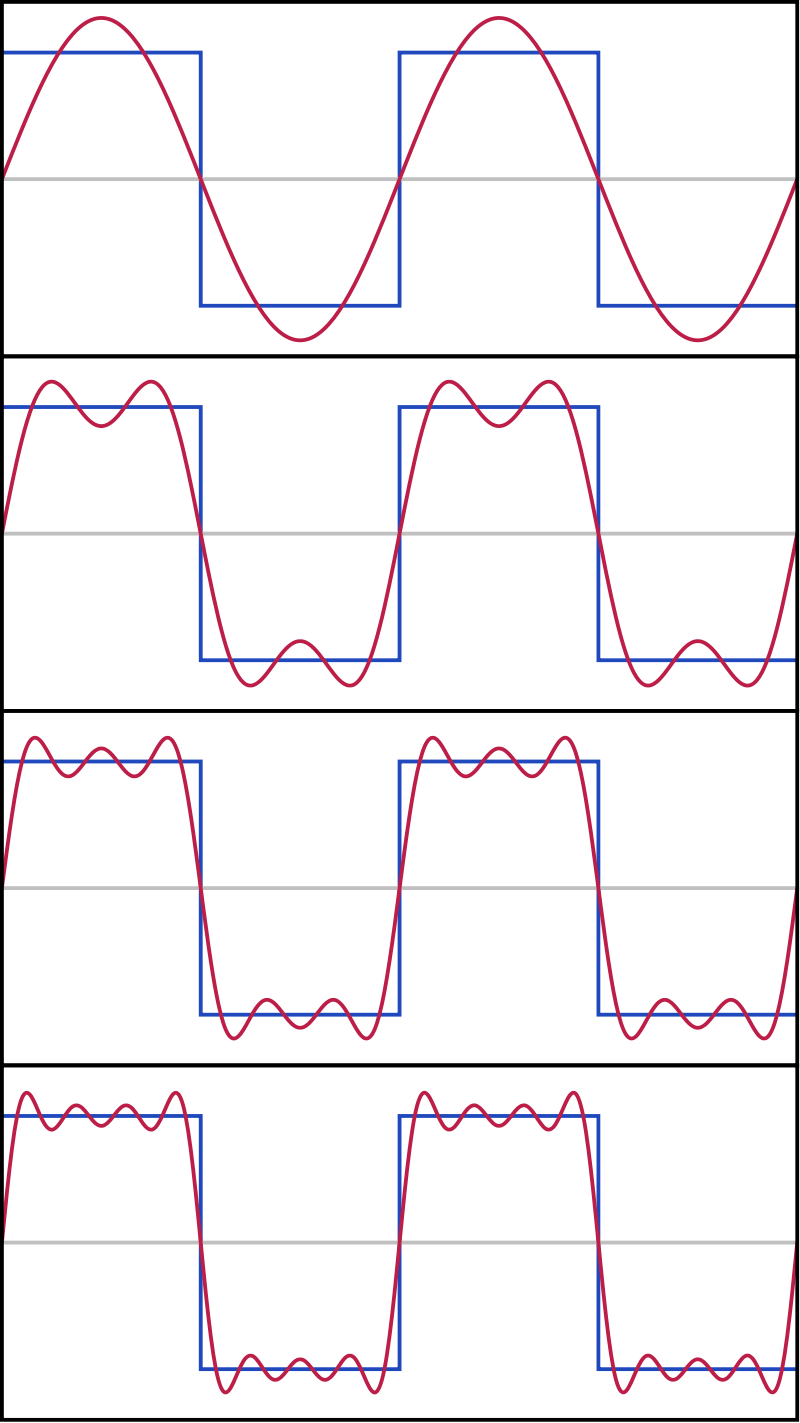
\includegraphics[height=2.5in]{exp/squarewave.png}}
\end{frame}

\begin{frame}
  \frametitle{Spectrum: Delayed Square Wave}
  Anyway, here's the square wave, after being delayed by the pure-delay filter:
  \centerline{\includegraphics[height=2.5in]{exp/delayedsquarewave.png}}
  You can see that magnitude's unchanged, but phase is changed.
\end{frame}

%%%%%%%%%%%%%%%%%%%%%%%%%%%%%%%%%%%%%%%%%%%%
\section[Cascades]{Cascaded LTI Systems}
\setcounter{subsection}{1}

\begin{frame}
  \frametitle{Output of a filter in response to a periodic signal}

  Suppose the input to a signal is periodic, $x[n+N]=x[n]$.  That
  means the signal is made up of pure tones, at multiples of the
  fundamental:
  \[
  x[n] = \frac{1}{N}\sum_{k=0}^{N-1} X[k] e^{jnk\omega_0}
  \]
  Therefore, if we pass it through a filter,
  \[
  y[n]=g[n]\ast x[n],
  \]
  we get:
  \[
  y[n]=\frac{1}{N}\sum_{k=0}^{N-1} Y[k] e^{jnk\omega_0},~~~Y[k]=G(k\omega_0)X[k]
  \]
\end{frame}

\begin{frame}
  \frametitle{Cascaded filters}

  Suppose I pass the signal through filter $g[n]$, then pass it through
  another filter, $f[n]$:
  \[
  y[n]=f[n]\ast \left(g[n]\ast x[n]\right),
  \]
  we get a signal $y[n]$ whose spectrum is:
  \[
  Y[k]=F(k\omega_0) G(k\omega_0) X[k]
  \]
\end{frame}

\begin{frame}
  \frametitle{Convolution  is commutative and associative}

  You know that multiplication is both commutative and associative.
  If $H(\omega)=F(\omega)G(\omega)$, then
  \[
  Y[k] = F(k\omega_0) G(k\omega_0) X[k]=G(k\omega_0)F(k\omega_0) X[k]=H(k\omega_0)X[k]
  \]
  and therefore:
  \[
  y[n]=f[n]\ast \left(g[n]\ast x[n]\right)=g[n]\ast \left(f[n]\ast x[n]\right)
  =h[n]\ast x[n]
  \]
\end{frame}

\begin{frame}
  \frametitle{Example: Differenced Square Wave}

  Suppose we define $x[n]=$square wave, $g[n]=$ pure-delay filter, and
  $f[n]=$ first-difference filter.  Here's $f[n]\ast x[n]$:
  \centerline{\includegraphics[height=2.5in]{exp/differenced_squarewave.png}}
\end{frame}
\begin{frame}
  \frametitle{Example: Differenced Square Wave}

  Suppose we define $x[n]=$square wave, $g[n]=$ pure-delay filter, and
  $f[n]=$ first-difference filter.  Here's $f[n]\ast x[n]$:
  \centerline{\includegraphics[height=1.5in]{exp/differenced_squarewave.png}}
  You can see that the differencing operation has raised the amplitude
  of the higher harmonics, because the first-difference filter is a
  high-pass filter, as you saw last time.
\end{frame}

\begin{frame}
  \frametitle{Example: Delayed Differenced Square Wave}

  Here's $g[n]\ast f[n]\ast x[n]$, the delayed differenced square wave:
  \centerline{\includegraphics[height=2.5in]{exp/delayed_differenced_squarewave.png}}
  Again, the delay operation has changed the phases, but not the magnitudes.
\end{frame}

\begin{frame}
  \frametitle{Example: Differenced Delayed Square Wave}

  Here's $f[n]\ast g[n]\ast x[n]$, the differenced delayed square wave
  (hint: it's exactly the same as the previous slide!!)
  \centerline{\includegraphics[height=2.5in]{exp/differenced_delayed_squarewave.png}}
\end{frame}

\begin{frame}
  \frametitle{Magnitude and Phase of Cascaded Frequency Responses}

  Notice, in the previous two slides, that the magnitudes multiply:
  \[
  |H(\omega)|=|F(\omega)||G(\omega)|,
  \]
  but the phases add:
  \[
  \angle H(\omega) = \angle F(\omega)+\angle G(\omega).
  \]
  That's because:
  \[
  F(\omega)G(\omega)=|F(\omega)|e^{j\angle F(\omega)}|G(\omega)|e^{j\angle G(\omega)}
  =|F(\omega)||G(\omega)| e^{j\left(\angle F(\omega)+\angle G(\omega)\right)}
  \]
\end{frame}

%%%%%%%%%%%%%%%%%%%%%%%%%%%%%%%%%%%%%%%%%%%%
\section[Sum]{The Running-Sum Filter (Local Averaging)}
\setcounter{subsection}{1}

\begin{frame}
  \frametitle{Local Average Filters}

  Let's go back to the local averaging filter from Lecture 2. I want to define two 
  different types of local average: centered, and delayed.
  \begin{itemize}
  \item {\bf Centered local average:} This one averages
    $\left(\frac{L-1}{2}\right)$ future samples,
    $\left(\frac{L-1}{2}\right)$ past samples, and $x[n]$:
    \[
    y_c[n] = \frac{1}{L}\sum_{m=-\left(\frac{L-1}{2}\right)}^{\left(\frac{L-1}{2}\right)} x[n-m]
    \]
  \item {\bf Delayed local average:} This one averages $x[n]$ and $L-1$ of its
    past samples:
    \[
    y_d[n] = \frac{1}{L}\sum_{m=0}^{L-1} x[n-m]
    \]
  \end{itemize}
  Notice that $y_d[n] = y_c\left[n-\left(\frac{L-1}{2}\right)\right]$.
\end{frame}

\begin{frame}
  \frametitle{Local Average Filters}

  We can write both of these as filters:
  \begin{itemize}
  \item {\bf Centered local average:}
    \begin{align*}
      y_c[n] &= f_c[n]\ast x[n]\\
      f_c[n] &= \begin{cases} \frac{1}{L}& -\left(\frac{L-1}{2}\right)\le n\le\left(\frac{L-1}{2}\right)\\
        0&\mbox{otherwise}\end{cases}
    \end{align*}
  \item {\bf Delayed local average:}
    \begin{align*}
      y_d[n] &= f_d[n]\ast x[n]\\
      f_d[n] &= \begin{cases} \frac{1}{L}& 0\le n\le L-1\\
        0&\mbox{otherwise}\end{cases}
    \end{align*}
  \end{itemize}
\end{frame}

\begin{frame}
  \frametitle{Local Average Filters}
  \centerline{\includegraphics[height=2.5in]{exp/localaveragefilters.png}}
  Notice that $f_d[n]=f_c\left[n-\left(\frac{L-1}{2}\right)\right]$.
\end{frame}  

\begin{frame}
  \frametitle{The relationship between centered local average and delayed local average}

  Suppose we define our pure delay filter,
  \[
  g[n]=\delta\left[n-\frac{L-1}{2}\right] = \begin{cases}
  1 & n=\frac{L-1}{2}\\
  0 & \mbox{otherwise}
  \end{cases}
  \]
  Using $g[n]$, here are  lots of different ways we can write the relationship
  between $y_d[n]$, $y_c[n]$, and $x[n]$:
  \begin{align*}
    y_d[n] &= f_d[n]\ast x[n]\\
    y_c[n] &= f_c[n]\ast x[n]\\
    y_d[n] &= g[n]\ast y_c[n] = g[n]\ast f_c[n]\ast x[n]\\
    f_d[n] &= g[n]\ast f_c[n]
  \end{align*}
\end{frame}
  
\begin{frame}
  \frametitle{The relationship between centered local average and delayed local average}

  Remember the frequency response of a pure delay filter:
  \[
  G(\omega)  = e^{-j\omega\left(\frac{L-1}{2}\right)}
  \]
  We have not yet figured out what $F_c(\omega)$ and $F_d(\omega)$
  are.  But whatever they are, we know that
  \[
  f_d[n] = g[n]\ast f_c[n]
  \]
  and therefore
  \[
  F_d(\omega) = e^{-j\omega\left(\frac{L-1}{2}\right)} F_c(\omega)
  \]
\end{frame}
  
\begin{frame}
  \frametitle{The frequency response of a local average filter}

  Let's find the frequency response of
  \[
  f_d[n] = \begin{cases} \frac{1}{L}& 0\le m\le L-1\\
    0&\mbox{otherwise}\end{cases}
  \]
  The formula is
  \[
  F_d(\omega) = \sum_m f[m]e^{-j\omega m},
  \]
  so,
  \[
  F_d(\omega) = \sum_{m=0}^{L-1} \frac{1}{L}e^{-j\omega m}
  \]
\end{frame}
  
\begin{frame}
  \frametitle{The frequency response of a local average filter}

  \[
  F_d(\omega) = \sum_{m=0}^{L-1} \frac{1}{L}e^{-j\omega m}
  \]
  This is just a standard geometric series,
  \[
  \sum_{m=0}^{L-1} a^m = \frac{1-a^L}{1-a},
  \]
  so:
  \[
  F_d(\omega) = \frac{1}{L}\left(\frac{1-e^{-j\omega L}}{1-e^{-j\omega}}\right)
  \]
\end{frame}
  
\begin{frame}
  \frametitle{The frequency response of a local average filter}

  We now have an extremely  useful transform pair:
  \[
  f_d[n] = \begin{cases} \frac{1}{L}& 0\le m\le L-1\\
    0&\mbox{otherwise}\end{cases}~~~\leftrightarrow~~~
  F_d(\omega) = \frac{1}{L}\left(\frac{1-e^{-j\omega L}}{1-e^{-j\omega}}\right)
  \]
  Let's attempt to convert that into polar form, so we can find
  magnitude and phase response. Notice that both the numerator and the
  denominator are subtractions of complex numbers, so we might be able
  to use $2j\sin(x)=e^{jx}-e^{-jx}$ for some $x$.  Let's try:
  \begin{align*}
    \frac{1}{L}\left(\frac{1-e^{-j\omega L}}{1-e^{-j\omega}}\right)
    &= \frac{1}{L}\frac{e^{-j\omega L/2}}{e^{-j\omega/2}}
    \left(\frac{e^{j\omega L/2}-e^{-j\omega L/2}}{e^{j\omega/2}-e^{-j\omega/2}}\right)\\
    &= e^{-j\omega\left(\frac{L-1}{2}\right)}\frac{1}{L}
    \left(\frac{2j\sin(\omega L/2)}{2j\sin(\omega/2)}\right)\\
    &= e^{-j\omega\left(\frac{L-1}{2}\right)}\frac{1}{L}
    \left(\frac{\sin(\omega L/2)}{\sin(\omega/2)}\right)
  \end{align*}
\end{frame}
  
\begin{frame}
  \frametitle{The frequency response of a local average filter}

  Now we have $F_d(\omega)$ in almost magnitude-phase form:
  \[
  f_d[n] = \begin{cases} \frac{1}{L}& 0\le m\le L-1\\
    0&\mbox{otherwise}\end{cases}~~~\leftrightarrow~~~
  F_d(\omega)=\left(\frac{\sin(\omega L/2)}{L\sin(\omega/2)}\right)e^{-j\omega\left(\frac{L-1}{2}\right)}
  \]
  By the way, remember we discovered that
  \[
  f_d[n]=g[n]\ast f_c[n]~~~\leftrightarrow~~~F_d(\omega)=e^{-j\omega\left(\frac{L-1}{2}\right)}F_c(\omega)
  \]
  Notice anything?
\end{frame}

\begin{frame}
  \frametitle{Dirichlet form}

  The textbook calls this function the ``Dirichlet form:''
  \[
  D_L(\omega) = \frac{\sin(\omega L/2)}{\sin(\omega/2)}
  \]
  That is, exactly, the frequency response of a centered local sum filter:
  \[
  d_L[n] = \begin{cases}
    1 & -\left(\frac{L-1}{2}\right)\le n\le \left(\frac{L-1}{2}\right)\\
    0 & \mbox{otherwise}
  \end{cases}
  \]
\end{frame}

\begin{frame}
  \frametitle{Dirichlet form}

  Here's what it looks like:
  \centerline{\includegraphics[height=2.5in]{exp/dirichletform.png}}
\end{frame}
  
\begin{frame}
  \frametitle{Dirichlet form}

  Since every local averaging filter is based on Dirichlet form, it's
  worth spending some time to understand it better.
  \[
  D_L(\omega) = \frac{\sin(\omega L/2)}{\sin(\omega/2)}
  \]
  \begin{itemize}
  \item It's equal to zero every time $\omega L/2$ is a multiple of $\pi$.  So
    \[
    D_L\left(\frac{2\pi k}{L}\right)  = 0~~\mbox{for all integers}~k~\mbox{except}~k=0
    \]
  \item At $\omega=0$, the value of $\frac{\sin(\omega
    L/2)}{\sin(\omega/2)}$ is undefined, but it's posssible to prove
    that $\lim_{\omega\rightarrow 0}D_L(\omega)=L$.  To make life
    easy, we'll just define it that way:
    \[
    \mbox{DEFINE:}~~D_L(0)=L
    \]
  \end{itemize}
\end{frame}

\begin{frame}
  \frametitle{Dirichlet form}

  Here's what it looks like:
  \centerline{\includegraphics[height=2.5in]{exp/dirichletform.png}}
\end{frame}
  
\begin{frame}
  \frametitle{Local averaging filter}

  Here's what the centered local averaging filter looks like.  Notice that
  it's just $1/L$ times the Dirichlet form:
  \centerline{\includegraphics[height=2.5in]{exp/centeredaveragingfilter.png}}
\end{frame}
  
%%%%%%%%%%%%%%%%%%%%%%%%%%%%%%%%%%%%%%%%%%%%
\section[Denoising]{Denoising a Periodic Signal}
\setcounter{subsection}{1}

\begin{frame}
  \frametitle{Output of a filter in response to a periodic signal}

  Suppose the input to a signal is periodic, $x[n+N]=x[n]$.  That
  means the signal is made up of pure tones, at multiples of the
  fundamental:
  \[
  x[n] = \frac{1}{N}\sum_{k=0}^{N-1} X[k] e^{jnk\omega_0}
  \]
  Therefore, if we pass it through a filter,
  \[
  y[n]=g[n]\ast x[n],
  \]
  we get:
  \[
  y[n]=\frac{1}{N}\sum_{k=0}^{N-1} Y[k] e^{jnk\omega_0},~~~Y[k]=G\left(\frac{2\pi k}{N}\right)X[k]
  \]
\end{frame}

\begin{frame}
  \frametitle{Output of a local averaging filter in response to a periodic signal}

  What if we use a local averaging filter, averaging over one complete
  period of $x[n]$?
  \[
  y[n] = f_c[n]\ast x[n]
  \]
  \[
  f_c[n] = \begin{cases}
    \frac{1}{N} & -\left(\frac{N-1}{2}\right)\le n\le \left(\frac{N-1}{2}\right)\\
    0 & \mbox{otherwise}
  \end{cases}~~~\leftrightarrow~~~
  F_c(\omega)=\frac{\sin(\omega N/2)}{N\sin(\omega/2)}
  \]
  We get:
  \[
  Y[k]=F_c\left(\frac{2\pi k}{N}\right)X[k]=0!!!
  \]
\end{frame}

\begin{frame}
  \frametitle{Local averaging of a periodic signal: Time domain}

  \centerline{\animategraphics[loop,controls,height=2.5in]{5}{exp/localaverage_periodic}{0}{54}}
\end{frame}

\begin{frame}
  \frametitle{Local averaging of a periodic signal: Frequency domain}

  \centerline{\includegraphics[height=2.5in]{exp/localaverage_spectrum.png}}
\end{frame}

\begin{frame}
  \frametitle{Local averaging of a periodic signal}

  \begin{itemize}
  \item If you compute the average of a periodic signal, over one complete period
    the average is zero (assuming that there is no DC offset).
  \item What's left in $y[n]=f_c[n]\ast x[n]$ is just the background noise.
  \end{itemize}
\end{frame}

\begin{frame}
  \frametitle{A noisy signal}

  Here's a noisy signal:
  \centerline{\includegraphics[height=2.5in]{exp/noisysignal.png}}
\end{frame}

\begin{frame}
  \frametitle{A noise-only signal!}

  Here's a noisy signal, averaged over each period.  Notice, all that's left in $y[n]$ is the noise!
  \centerline{\animategraphics[loop,controls,height=2.5in]{5}{exp/noised_signal}{0}{54}}
\end{frame}

\begin{frame}
  \frametitle{Local averaging of a periodic signal}

  \begin{itemize}
  \item If you compute the average of a periodic signal, over one complete period
    the average is zero (assuming that there is no DC offset).
  \item What's left in $y[n]=f_c[n]\ast x[n]$ is just the background noise.
  \item Can we subtract the background noise from the original signal?
    \[
    z[n] = x[n] - y[n]
    \]
    Would that give us a version of $x[n]$ with less background noise?
  \end{itemize}
\end{frame}

\begin{frame}
  \frametitle{Local averaging of a periodic signal}

  \begin{itemize}
  \item The noisy signal is
    \[
    x[n] = \delta[n]\ast x[n]
    \]
  \item Noise is all that's left after we get rid of the periodic part, using
    \[
    y[n]=f_c[n]\ast x[n]
    \]
  \item Can we subtract the background noise from the original signal?
    \[
    z[n] = x[n] - y[n] = (\delta[n]-f_c[n])\ast x[n]
    \]
  \end{itemize}
\end{frame}

\begin{frame}
  \frametitle{A denoising  filter}

  So the de-noising filter is:
  \[
  h[n] = \delta[n]-f_c[n]
  \]
\end{frame}

\begin{frame}
  \frametitle{Denoising filter}

  Here are the delta function, local averaging filter, and denoising filter in the time domain:
  \centerline{\includegraphics[height=2.5in]{exp/denoising_impulseresponse.png}}
\end{frame}

\begin{frame}
  \frametitle{Denoising filter}

  Here are the delta function, local averaging filter, and denoising filter in the frequency domain:
  \centerline{\includegraphics[height=2.5in]{exp/denoising_frequencyresponse.png}}
\end{frame}

\begin{frame}
  \frametitle{A denoised signal}

  Here's a denoised signal:
  \centerline{\animategraphics[loop,controls,height=2.5in]{5}{exp/denoised_signal}{0}{54}}
\end{frame}

\begin{frame}
  \frametitle{A denoised signal}

  Here's the noisy and denoised signals in the frequency domain:
  \centerline{\includegraphics[height=2.5in]{exp/denoised_spectrum.png}}
\end{frame}

\begin{frame}
  \frametitle{Not a very good denoising filter?}

  OK, so that wasn't really a very {\bf good} denoising filter!
  Can we do better?
  \ldots wait until after the midterm, and we'll talk about how to do better\ldots
\end{frame}

%%%%%%%%%%%%%%%%%%%%%%%%%%%%%%%%%%%%%%%%%%%%
\section[Summary]{Summary}
\setcounter{subsection}{1}

\begin{frame}
  \frametitle{Summary}
  \begin{itemize}
  \item The {\bf Pure Delay Filter} has $|G(\omega)|=1$, $\angle G(\omega)=-\omega n_0$:
    \[
    g[m]=\delta[n-n_0]~~~\leftrightarrow~~~G(\omega) = e^{-j\omega n_0}
    \]
  \item {\bf Cascaded LTI Systems} convolve their impulse responses, equivalently, they
    multiply their frequency responses:
    \[
    h[n]=f[n]\ast g[n]~~~\leftrightarrow~~~H(\omega)=F(\omega)G(\omega)
    \]
  \item The {\bf Centered Local Averaging Filter} is $1/L$ times
    the Dirichlet form:
    \[
    f_c[n] = \begin{cases}
      \frac{1}{L} & -\left(\frac{L-1}{2}\right)\le n\le \left(\frac{L-1}{2}\right)\\
      0 & \mbox{otherwise}
    \end{cases}~~~\leftrightarrow~~~
    F_c(\omega)=\frac{\sin(\omega L/2)}{L\sin(\omega/2)}
    \]
  \item The {\bf Delayed Local Averaging Filter} is $f_c[n]$, delayed by half of its length:
    \[
    f_d[n] = \begin{cases}
      \frac{1}{L} & 0\le n\le L-1\\
      0 & \mbox{otherwise}
    \end{cases}~~~\leftrightarrow~~~
    F_d(\omega)=\frac{\sin(\omega L/2)}{L\sin(\omega/2)}e^{-j\omega\left(\frac{L-1}{2}\right)}
    \]
  \end{itemize}
\end{frame}

\end{document}
